\documentclass{article}

\usepackage{amsmath,amssymb,graphicx}
\usepackage[parfill]{parskip}
\usepackage{hyperref}

\AtBeginEnvironment{quote}{\par\small}


\begin{document}

{
	\centering
	\section*{Extragalactic Astrophysics HW3}
	Connor Hainje
	\vspace{2em}
	\par
}

For this homework, I've decided to do \textbf{Detectors, Analytic Exercise
\#2}. Here is the problem statement.

\begin{quote}
It is a commonly used practice to combine different observations of a quantity
(say flux) by using a weighted mean, using weights equal to the inverse
variance of each observation. The advantage of doing so is that if the inverse
variance is known, this weighted mean is the minimum variance estimator of the
quantity itself. For imaging conducted with photon counting detectors, when the
background is minimal, the noise in a data set is the Poisson noise in the
expectation value of the signal. However, observationally we often only have
access to one realization of the signal, and often the quoted errors are based
on the Poisson noise estimated from the signal itself. If we take multiple
observations and combine them together weighting by the inverse variance
estimated in this way, it leads to a bias. Ignoring any background contribution
to the noise, estimate this bias as a function of the true expected number of
photons $\bar n$.
\end{quote}



Suppose we have observations $n_i$ which are sampled from a Poisson
distribution of true mean $\bar n$. What is the signal we estimate from these
observations if we take the noise estimate for each observation to be
$\sigma_i^2 = n_i$?

As in the problem statement, we combine the observations by a weighted mean,
with observations weighted by the inverse variance. The combined signal
estimate is then given by
\begin{align}
	\text{signal}
	&= \frac{\sum_i n_i \sigma_i^{-2}}{\sum_i \sigma_i^{-2}} \\
	&= \frac{\sum_i n_i n_i^{-1}}{\sum_i n_i^{-1}} \\
	&= \frac{N}{\sum_i n_i^{-1}} \\
	&= \left( \frac{1}{N} \sum_i n_i^{-1} \right)^{-1}
\end{align}
The bias is given by $\text{signal} - \bar n$. We can find the expected value
of the bias by computing the expected value of the signal, given that $n_i$ are
observations of random variable $n \sim \text{Pois}(\bar n)$. Note then that
the signal above is an estimate of
\begin{equation}
	\left( \mathbb{E}[n^{-1}] \right)^{-1}
\end{equation}
which we can compute. This expectation value is given by
\begin{align}
	\mathbb{E}[n^{-1}]
	&= \sum_{k=0}^{\infty} \left(\frac{1}{k}\right) \frac{\bar{n}^k e^{-\bar{n}}}{k!} \\
	&= e^{-\bar{n}} \sum_{k=0}^{\infty} \frac{\bar{n}^k}{k \ k!}.
\end{align}
As stated, this is ill posed, as the summand contains $1 / 0$ for $k = 0$. We'll try
to patch this up by assuming $\sigma_i^2 = 1$ if $n_i = 0$, but this will probably
cause us to incur an error. Making this substitution, we have
\begin{align}
	\mathbb{E}[n^{-1}]
	&= e^{-\bar{n}} \sum_{k=0}^{\infty} \frac{\bar{n}^k}{k \ k!} \\
	&= e^{-\bar{n}} \left[1 + \sum_{k=1}^{\infty} \frac{\bar{n}^k}{k \ k!}\right].
\end{align}
Mathematica allows us to evaluate the series, obtaining
\begin{equation}
	\sum_{k=1}^{\infty} \frac{\bar{n}^k}{k \ k!}
	=
	-\gamma + \text{Ei}(\bar n) - \log (\bar n),
\end{equation}
where $\gamma$ is the Euler Gamma constant ($\gamma \approx 0.577$) and
$\text{Ei}$ is the exponential integral function.
Hence, the expected bias can be written
\begin{align}
	\text{bias}
	&= \left( \mathbb{E}[n^{-1}] \right)^{-1} - \bar n \\
	&= \left( e^{-\bar{n}} \left[1 - \gamma + \text{Ei}(\bar n) - \log (\bar n)\right] \right)^{-1} - \bar n \\
	&= \frac{e^{\bar{n}}}{1 - \gamma + \text{Ei}(\bar n) - \log (\bar n)} - \bar n.
\end{align}
We can plot this for a range of $\bar n$ values. The result is shown in
Figure~\ref{fig:analytic}. The figure shows that the bias starts at 1 and
decreases sharply with $\bar n$ until around $\bar n \sim 6$, after which is
plateaus around $-1$.

\begin{figure}
	\begin{center}
		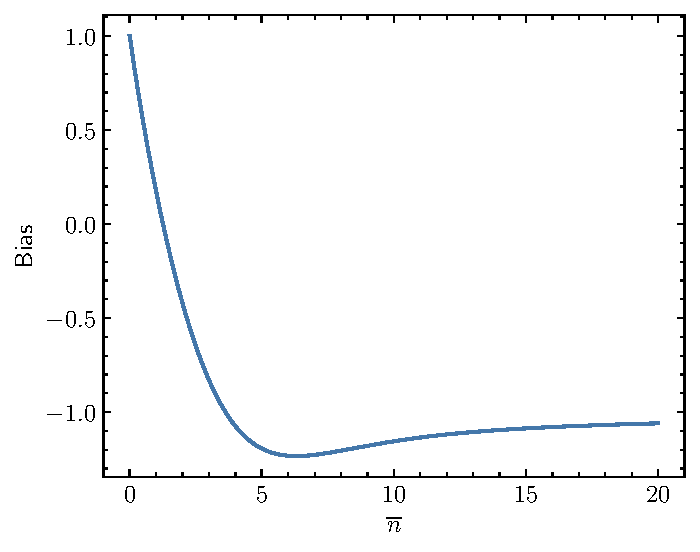
\includegraphics[width=0.7\textwidth]{figures/analytic_estimate.pdf}
	\end{center}
	\caption{%
		Analytic estimate of the expected bias for a range of the true
		mean $\bar n$.
	}
	\label{fig:analytic}
\end{figure}

We can also estimate the bias numerically. We'll do this as follows.

\begin{itemize}
	\item Given a value of $\bar n$, draw 1\,000 samples from
		$\text{Pois}(\bar n)$.
	\item Assign each sample a variance estimate $\sigma_i^2 = \max(n_i,
		1)$ and compute the bias of the combined signal estimate
		$\text{bias} = \sum_i n_i \sigma_i^{-2} / \sum_i \sigma_i^{-2}
		- \bar n$.
	\item Repeat this procedure 1\,000 times to get 1\,000 estimates of the
		bias, and take the median of the resulting distribution.
	\item Repeat for additional values of $\bar n$.
\end{itemize}


Carrying out this procedure for 20 values of $\bar n$ between $10^{-4}$ and 20
(using $10^{-4}$ to avoid divisions by zero) gives a plot of median numerical
bias versus $\bar n$, which is shown in Figure~\ref{fig:numerical}. Plotted
alongside these results are the numerical estimates.

\begin{figure}
	\begin{center}
		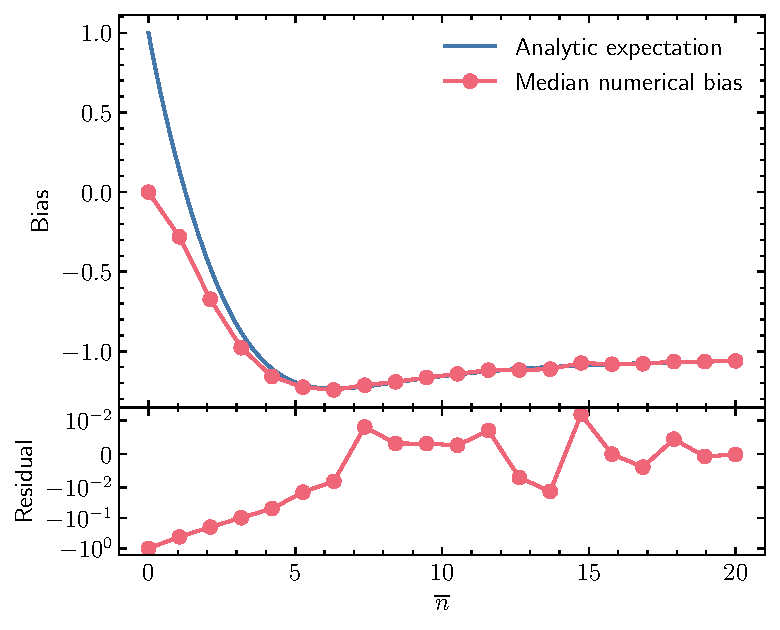
\includegraphics[width=0.8\textwidth]{figures/numerical_estimate.pdf}
	\end{center}
	\caption{%
		Numerical bias estimate computed by drawing samples from
		Poisson distributions many times and computing the actual
		average bias from combining the signals in the given way. Also
		plotted is the same curve as Figure~\ref{fig:analytic} for
		comparison. The two methods agree well for $\bar n \gtrsim 6$,
		but disagree strongly at small $\bar n$.
	}
	\label{fig:numerical}
\end{figure}

We see that for $\bar n \gtrsim 6$, the two methods agree to better than a
percent, supporting our calculation. For small $\bar n$, though, we become
sensitive to the $n_i = 0$ issue, and the two methods diverge.

This is because using a value of $\sigma_i^2 = 1$ when $n_i = 0$ (as is done in
the numerical estimate) is somewhat different from computing 
\begin{equation}
\mathbb{E}[1/n] \approx \sum_{k=0}^{\infty} P(k|\overline n) \ \text{max}(k,1)^{-1},
\end{equation}
as this second one is actually changing the $n_i = 0 \to 1$ as well. We can
verify this by re-running the numerical estimate, and setting both $n_i$ and
$\sigma_i^2$ to $1$ whenever our sample of $n_i = 0$. The result is given in
Figure~\ref{fig:difference} and verifies the claim. In this way, the numerical
estimate is probably ``more'' correct, as it makes a weaker assumption about
what to do when $n_i = 0$.

\begin{figure}
	\begin{center}
		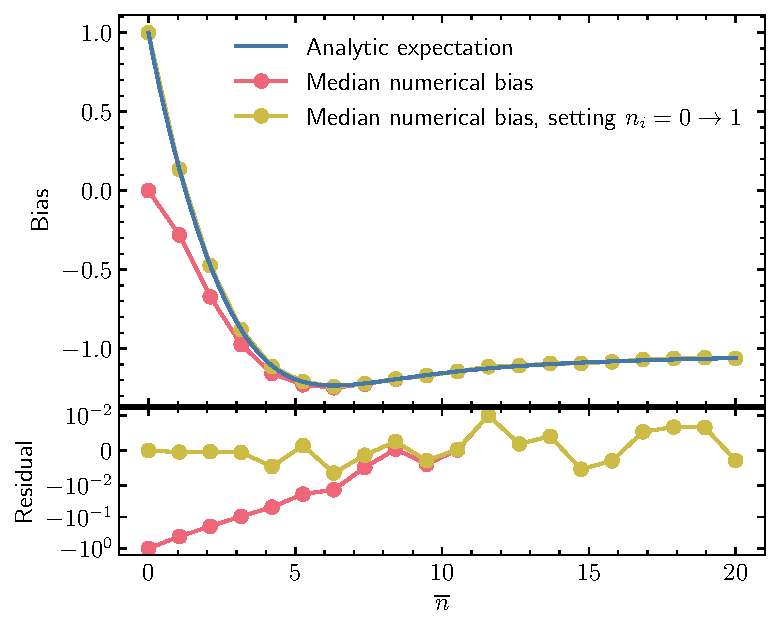
\includegraphics[width=0.8\textwidth]{figures/difference_explanation.pdf}
	\end{center}
	\caption{%
		Figure~\ref{fig:numerical} reproduced with an additional curve
		showing the result of setting all samples $n_i = 0$ to 1 (not
		just their associated variance estimates). This verifies that 
		the difference between our analytic and numerical estimates is
		due to this, and as such the numerical estimate is ``more''
		correct, probably.
	}
	\label{fig:difference}
\end{figure}

The code is available online at the following links: \href{https://github.com/cmhainje/exgal-hw/blob/main/hw3/series.nb}{Mathematica notebook}
and \href{https://github.com/cmhainje/exgal-hw/blob/main/hw3/numerics.ipynb}{Jupyter notebook}.


\end{document}
